\chapter{Methodology}


\section{Data set description}

The same data set as Wu et. al is used which is part of the publicly available 
benchmark data sets of MoleculeNet.\cite{wu2018moleculenet} This data set contains 
the measured solubility at $25^{\circ} C$ in $log(mol/L)$ for $1110$ compounds when duplicates 
are removed. Molecules are represented as a string using the simple molecular 
line entry system \big(SMILES\big).\cite{weininger1988smiles} Another representation 
of molecules is a graph where the atoms represent the nodes and the bonds represent 
the edges. Molecular graphs can be generated from SMILES using the python package 
rdkit (\cref{fig:smiles_and_graphs}).\cite{landrum2010r}


\begin{figure}[h]
    \centering
    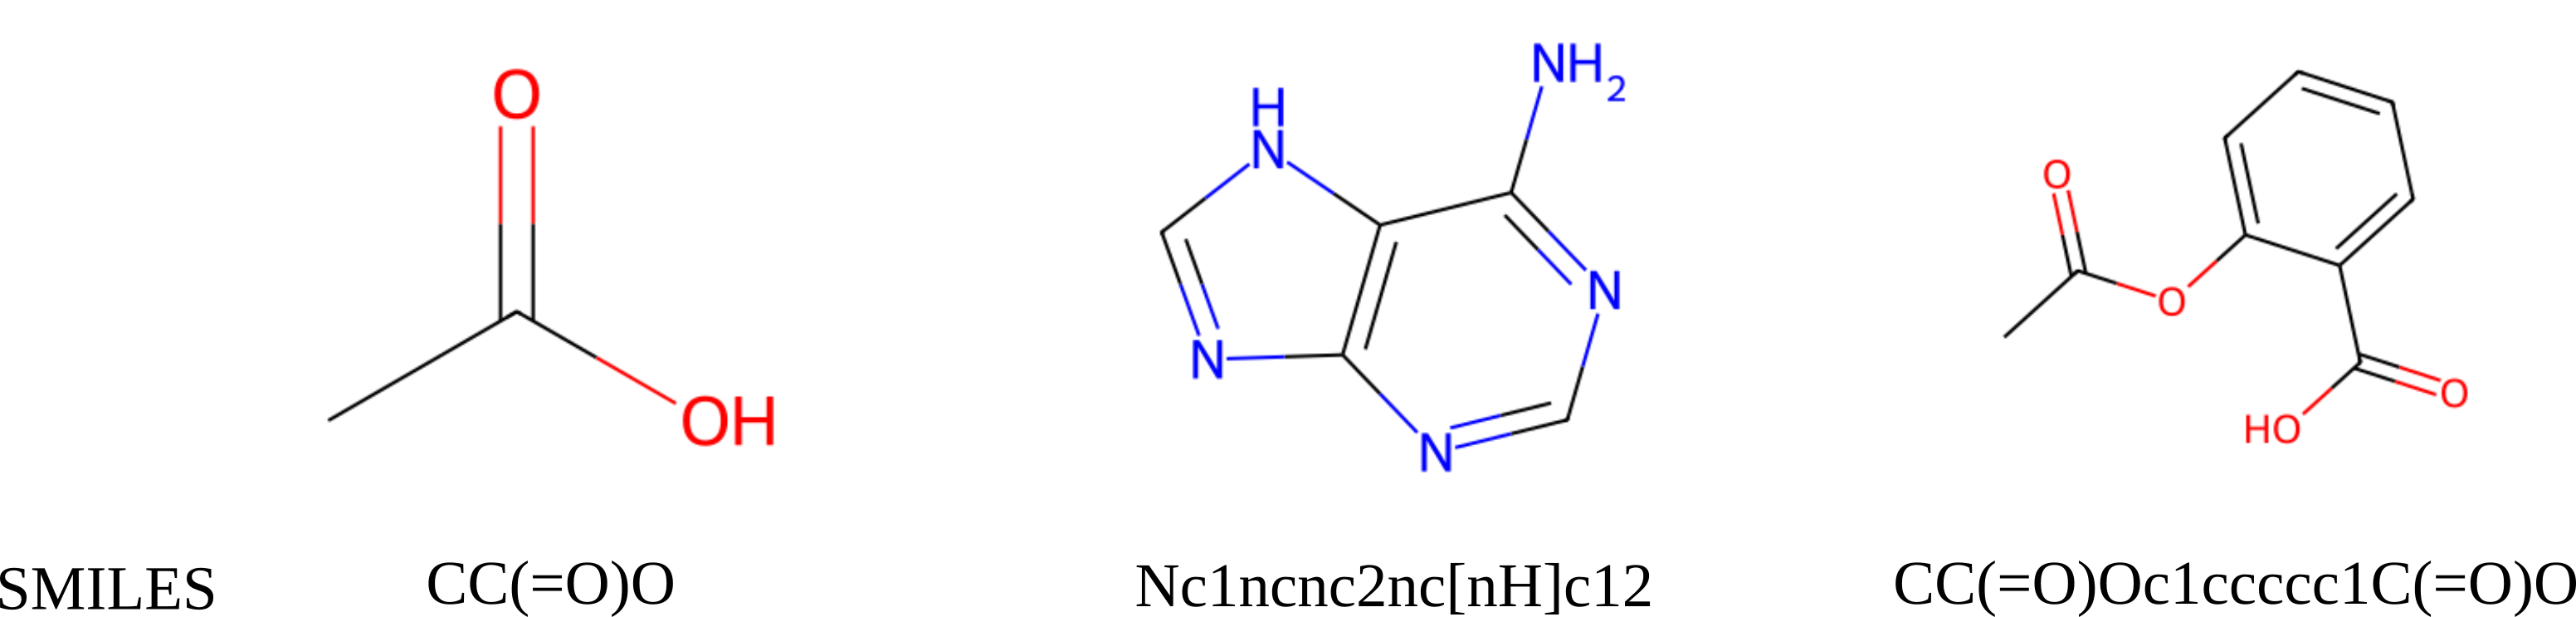
\includegraphics[scale=0.85]{smiles_to_graph_example.png}
    \caption{Examples of relationship between SMILES and molecular graphs for acetic acid (left),
    adenine (middle) and aspirin (right).}
    \label{fig:smiles_and_graphs}
\end{figure}



\section{Architecture of the graph neural network model to predict water solubility}
